\documentclass[tikz,border=2pt]{standalone}
\usepackage{amsmath}
\usepackage{amssymb}
\usepackage{xcolor}

\definecolor{journalink}{HTML}{1F1C18}
\definecolor{journalmuted}{HTML}{8A7F72}
\definecolor{journalaccent}{HTML}{9C2D2D}

\begin{document}
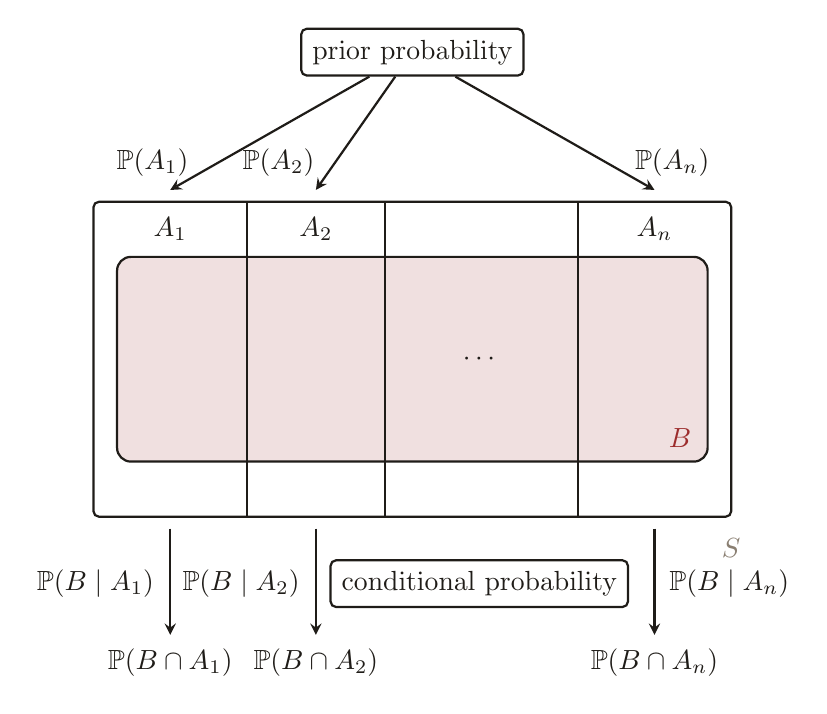
\begin{tikzpicture}[
  x=1cm,
  y=1cm,
  every node/.style={font=\normalsize},
  >=stealth
]
  % ---- sample space, partition strips and the event B ------------------
  \fill[journalaccent, fill opacity=0.15, rounded corners=5pt]
    (-3.75,-1.3) rectangle (3.75,1.3);

  \draw[journalink, line width=0.8pt, rounded corners=2pt]
    (-4.05,-2) rectangle (4.05,2);

  \draw[journalink, line width=0.8pt] (-2.10,-2) -- (-2.10,2);
  \draw[journalink, line width=0.8pt] (-0.35,-2) -- (-0.35,2);
  \draw[journalink, line width=0.8pt] (2.10,-2) -- (2.10,2);

  \draw[journalink, line width=0.8pt, rounded corners=5pt]
    (-3.75,-1.3) rectangle (3.75,1.3);

  \node[journalink] at (-3.075,1.65) {$A_1$};
  \node[journalink] at (-1.225,1.65) {$A_2$};
  \node[journalink] at (3.075,1.65) {$A_n$};
  \node[journalink] at (0.875,0) {$\cdots$};

  \node[journalaccent] at (3.40,-1) {$B$};
  \node[journalmuted] at (4.05,-2.4) {$S$};

  % ---- prior probabilities ---------------------------------------------
  \node[draw=journalink, line width=0.8pt, rounded corners=2pt,
        inner sep=4pt, journalink] (prior) at (0,3.9) {prior probability};

  \draw[journalink, line width=0.8pt, ->] (prior) -- (-3.075,2.15);
  \draw[journalink, line width=0.8pt, ->] (prior) -- (-1.225,2.15);
  \draw[journalink, line width=0.8pt, ->] (prior) -- (3.075,2.15);

  \node[journalink] at (-3.30,2.5) {$\mathbb{P}(A_1)$};
  \node[journalink] at (-1.70,2.5) {$\mathbb{P}(A_2)$};
  \node[journalink] at (3.30,2.5) {$\mathbb{P}(A_n)$};

  % ---- conditional probabilities and intersection probabilities --------
  \node[draw=journalink, line width=0.8pt, rounded corners=2pt,
        inner sep=4pt, journalink] at (0.85,-2.85) {conditional probability};

  \draw[journalink, line width=0.8pt, ->] (-3.075,-2.15) -- (-3.075,-3.5);
  \draw[journalink, line width=0.8pt, ->] (-1.225,-2.15) -- (-1.225,-3.5);
  \draw[journalink, line width=0.8pt, ->] (3.075,-2.15) -- (3.075,-3.5);

  \node[journalink] at (-4.025,-2.85) {$\mathbb{P}(B\mid A_1)$};
  \node[journalink] at (-2.175,-2.85) {$\mathbb{P}(B\mid A_2)$};
  \node[journalink] at (4.025,-2.85) {$\mathbb{P}(B\mid A_n)$};

  \node[journalink] at (-3.075,-3.85) {$\mathbb{P}(B\cap A_1)$};
  \node[journalink] at (-1.225,-3.85) {$\mathbb{P}(B\cap A_2)$};
  \node[journalink] at (3.075,-3.85) {$\mathbb{P}(B\cap A_n)$};
\end{tikzpicture}
\end{document}
